%%%%%%%%%%%%%%%%%%%%%%%%%%%%%%%%%%%%%%%%%%%%%%%%%%%%%%%%%%%%%%%%%%%%%%%%
% Plantilla TFG/TFM
% Escuela Politécnica Superior de la Universidad de Alicante
% Realizado por: Jose Manuel Requena Plens
% Contacto: info@jmrplens.com / Telegram:@jmrplens
%%%%%%%%%%%%%%%%%%%%%%%%%%%%%%%%%%%%%%%%%%%%%%%%%%%%%%%%%%%%%%%%%%%%%%%%

\chapter{Experimentación}
\label{experimentacion}

En este punto del trabajo se va a mostrar toda la experimentación realizada en este proyecto con la red, para ello se va a comenzar comentando los arreglos que se hicieron necesarios para poder realizar la comparación de los modelos.

\section{Limpieza a los modelos obtenidos con la herramienta Tech4diet}

Los modelos generados por Tech4diet, tienen suciedad en la parte de los pies, pues representan la plataforma que pisas para hacerte la reconstrucción del cuerpo.

Este proceso fue necesario para tratar de tener una buena comparativa de modelos obtenidos por nuestra red, dado que hasta la alineación era compleja por este motivo. El proceso se realizó con la herramienta de Blender, se eliminaron las partes sobrantes como se puede ver en la siguiente imagen.

\begin{figure}[H]
	\centering
	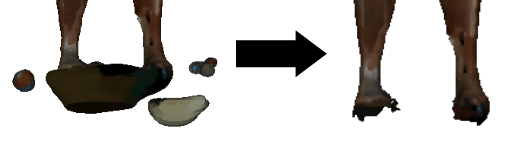
\includegraphics[scale=1]{imagenes/experimentacion1.png}
	\caption{Proceso limpieza modelo Tech4diet}
	\label{fig:figura9}
\end{figure}

Como se puede ver en la figura \ref{fig:figura9} se ha limpiado la plataforma, que no forma parte de nuestro cuerpo.


\section{Alineamiento de modelos}

La distancia de Hausdorff se va a calcular en MeshLab, para realizarla necesitamos alinear los modelos.

Este proceso se hace mediante la herramienta $Align$ dentro de MeshLab, de esta manera, aparece una ventana y alinearemos eligiendo $Point Based Glueling$, para ello antes se selecciona el modelo obtenido por Tech4diet y seleccionamos a $Glue Mesh Here$, esto se hace así porque es la que no queremos que cambie ni de ángulo ni nada en general.

Una vez seleccionada la opción para alinear nos saldrá una ventana en la que iremos eligiendo puntos en ambos modelos para poder alinearlos correctamente.

\begin{figure}[H]
	\centering
	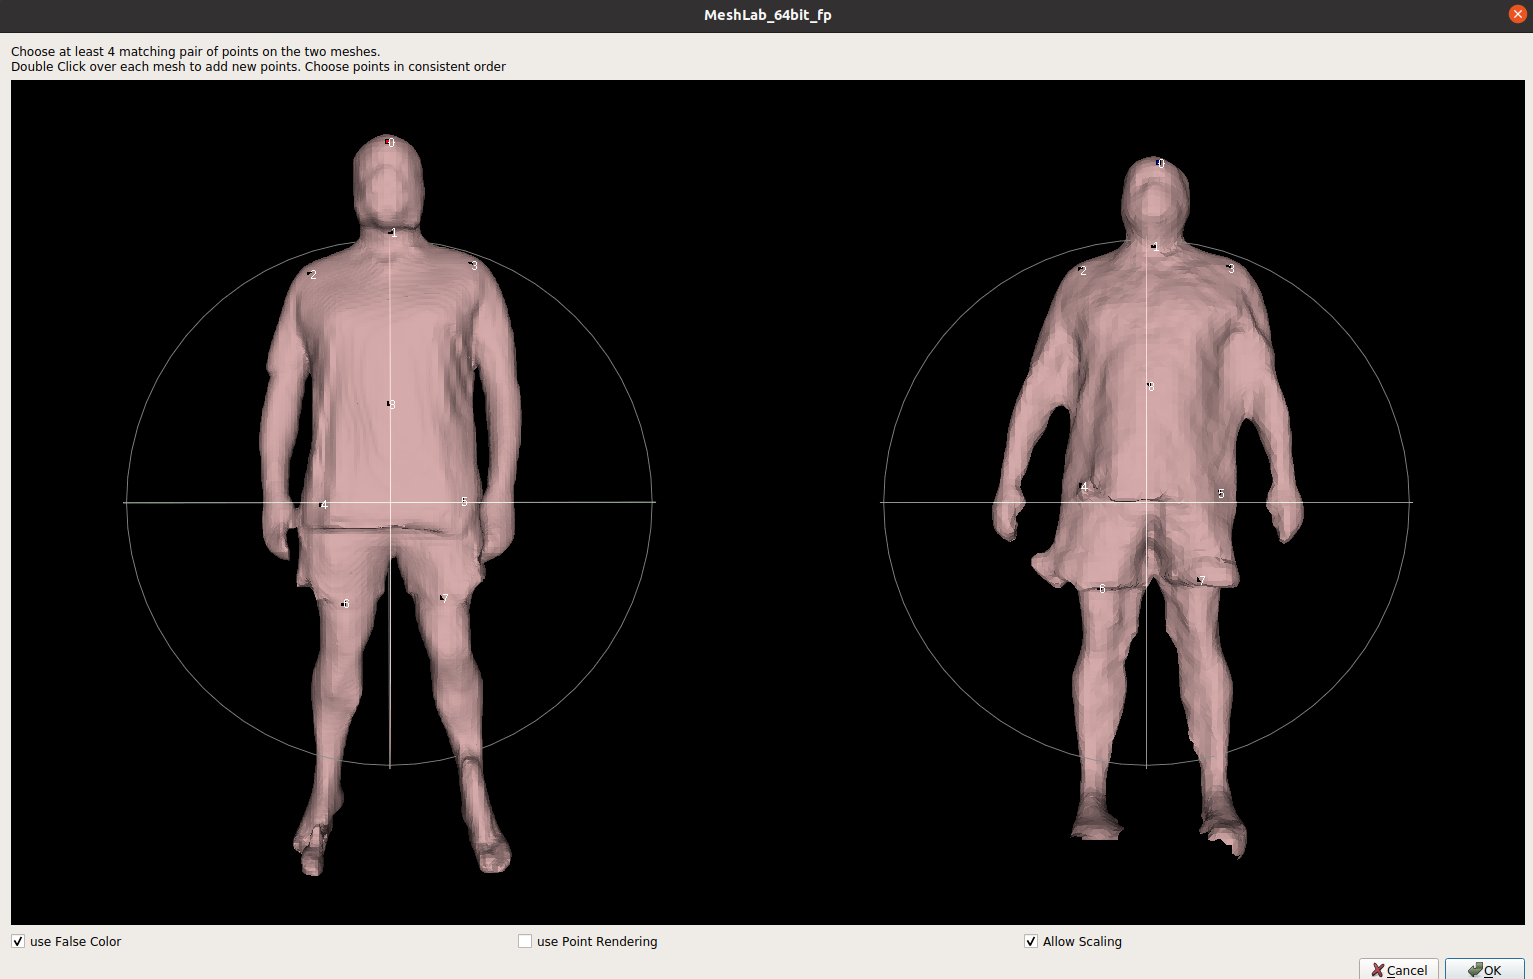
\includegraphics[scale=0.3]{imagenes/alineamiento.png}
	\caption{Proceso alineamiento modelos}
	\label{fig:figura10}
\end{figure}

En la figura \ref{fig:figura10} podemos observar dos modelos, el de la izquierda es el obtenido mediante la red, el de la derecha es el obtenido por Tech4diet

Una vez seleccionados los puntos correctamente y en estos caso seleccionado $Allow Scaling$ (esto lo he hecho porque la red no es capaz de que las medidas sean exactas a diferencia de Tech4diet), se realiza el alineamiento.

\begin{figure}[H]
	\centering
	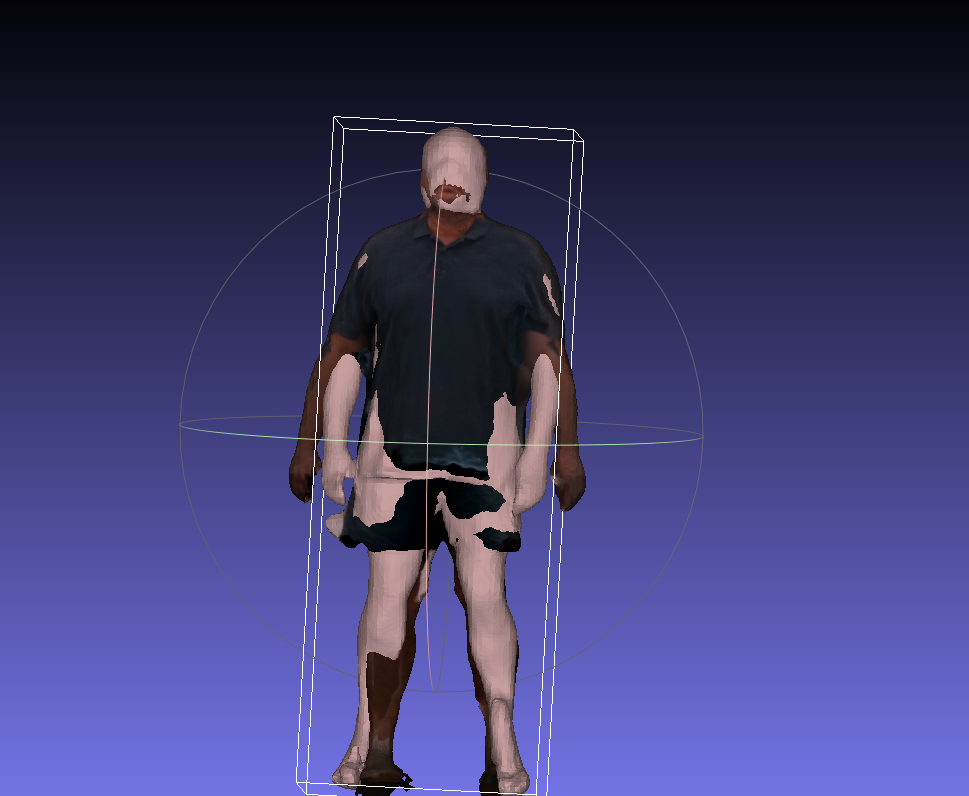
\includegraphics[scale=0.3]{imagenes/alineamiento2.png}
	\caption{Modelos alineados}
	\label{fig:figura11}
\end{figure}

En la figura \ref{fig:figura11} se observa el resultado obtenido después de la alineación.

Con la alineación realizada ya se puede usar la herramienta que nos calcula la distancia de Hausdorff.

\section{Creación de las nubes de punto correspondientes a cada modelo}

Para poder realizar el cálculo de la distancia de Chamfer es necesario tener las nubes de punto, porque las nubes de punto son $arrays$ con las coordenadas (también tienen la información del color y las normales, pero en este caso se va a eliminar esta información). Para ello se puede usar las aplicaciones MeshLab o CloudComparer.

He seleccionado CloudComparer, porque podías eliminar la información de los colores y de las normales desde la misma herramienta.

\section{Cálculo distancias}

Para poder comparar los modelos se han utilizado las distancias de Hausdorff y Chamfer como se ha mencionado con anterioridad, en este punto se va a explicar como se han obtenido las medidas.

\subsection{Distancia Hausdorff}
Como se ha comentado en el punto 4.1, la distancia de Hausdorff de ha calculado mediante la herramienta de MeshLab que te permite calcularla, esta te da un resultado parecido al siguiente: 

\begin{python}
	"Hausdorff Distance computed
	Sampled 58888 pts (rng: 0) on result_camelia0.obj searched closest on Camelia.obj
	min : 0.000000 max 0.339742 mean : 0.020914 RMS : 0.029951
	Values w.r.t. BBox Diag (1.819615)
	min : 0.000000 max 0.186711 mean : 0.011493 RMS : 0.016460"
\end{python}

Donde $min$ dignifica la mínima distancia que hay entre las mallas, $max$ la máxima distancia existente de un punto a otro de las mallas, $mean$ es la media y $RMS$ significa Root Mean Square, que es la raíz cuadrada de la media aritmética de los cuadrado de los valores.

Tenemos dos líneas de valores en la primera esta sobre la unidad de medida que en este caso es en metros, y la segunda línea son los valores anteriores obtenidos pero divididos por la longitud de la diagonal de la bounding box (cuadro delimitador de las mallas) de la malla que se usa como referencia, en este caso usamos la malla obtenida por Tech4diet.

\pagebreak
\subsection{Distancia Chamfer}
Por otro tenemos la distancia Chamfer, para ello se ha programado utilizado la siguiente función en python:

\begin{lstlisting}[caption={Código obtención distancia chamfer}, label=cod:3]
\end{lstlisting}
\begin{python}
	def chamfer_distance(x, y, metric='l2'):
		x_nn = NearestNeighbors(n_neighbors=1, leaf_size=1, algorithm='kd_tree', metric=metric).fit(x)
		min_y_to_x = x_nn.kneighbors(y)[0]
		y_nn = NearestNeighbors(n_neighbors=1, leaf_size=1, algorithm='kd_tree', metric=metric).fit(y)
		min_x_to_y = y_nn.kneighbors(x)[0]
		chamfer_dist = np.mean(min_y_to_x) + np.mean(min_x_to_y)
	return chamfer_dist
\end{python}

En el código \ref{cod:3} se calcula la distancia media mínima para cada punto que hay de la malla $x$ a la $y$ y viceversa.
\clearpage

\section{Comparativas}

Por un lado comentar que la red genera modelos del mismo tamaño sin importar la altura de la persona, este caso es importante y necesario que los tamaños sean los reales, por eso en la herramienta de alineamiento se seleccionó el escalado, pero a diferencia de eso, en la distancia de Chamfer no se ha podido mantener dicho escalado.

\begin{figure}[H]
	\centering
	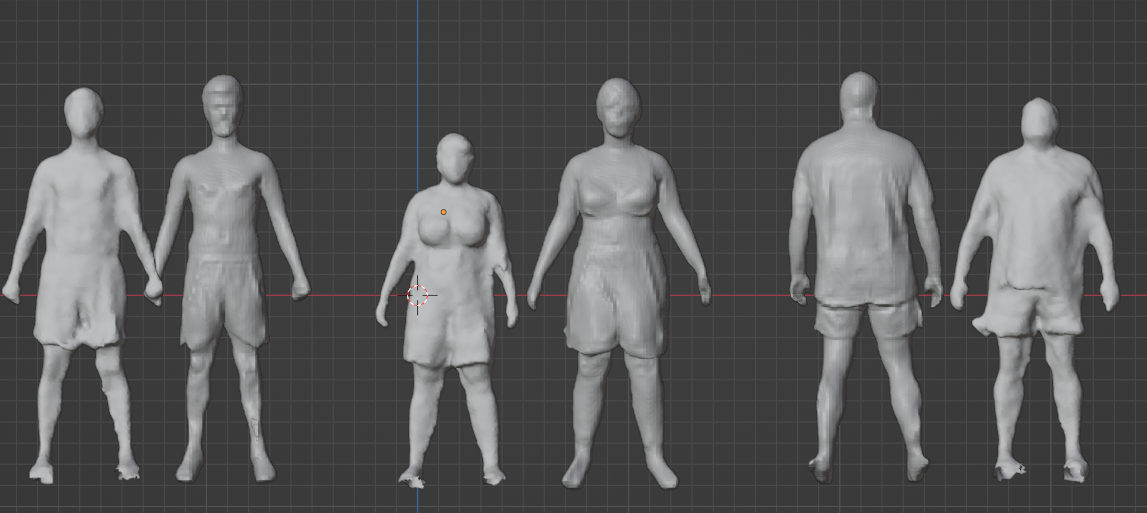
\includegraphics[scale=0.4]{imagenes/difaltura.png}
	\caption{Diferencia de altura de los modelos, el modelo más grande es el generado por la red}
	\label{fig:figura12}
\end{figure}






